% !TEX root = ../main.tex
\subsubsection{Hadronic Variables}
\label{14.22::hadronic_variables}
    The acceptance of the hadronic variables $z_h$, $p_T^2$, and $\phi_{PQ}$ for $e^-\pi^+$ and $e^-\pi^-$ is presented in Figure \ref{fig::14.22::hadronic_acc}.
    Each plot shows the acceptance in an integrated kinematical region for all electron variables and other hadronic variables.

    % Lower acceptance.
    It can be observed from the figures that the acceptance for the hadronic variables is lower compared to that of the electron variables.
    This is expected since the detection of the hadronic variables requires both the trigger electron and at least one hadron to be detected by the CLAS12 detector.
    This effect is also reflected in the entries for $e^-\pi^+$ and $e^-\pi^-$ in the efficiency Table \ref{tab::14.14::fmt_efficiency_study}.

    % Particle charge-dependent acceptance.
    Furthermore, the acceptance for the hadronic variables is shown to be approximately half for $e^-\pi^-$ compared to $e^-\pi^+$.
    This difference is related to the $\theta$ acceptance of CLAS12, which is influenced by the non-trivial magnetic field of the solenoid.
    As explained in Section \ref{14.21::electron_variables}, during the majority of run 12016, the solenoid field was configured to a polarity of $-0.75$.
    This causes negative particle tracks to bend inward towards the low-$\theta$ region of the Drift Chambers (DC), while positive particle tracks bend outward towards the high-$\theta$ region.

    The $\phi$ and $\theta$ acceptances of the detector for negative particles can be seen in Figure \ref{fig::14.21::theta_study_neg}, whereas those for positive particles are shown in Figure \ref{fig::14.22::theta_study_pos}.
    These plots clearly demonstrate that the DC is generally more receptive to positive particles.
    Consequently, there is a higher detection efficiency for $\pi^+$ compared to $\pi^-$, which explains the differences in the acceptance of the hadronic variables between $e^-\pi^+$ and $e^-\pi^-$.

    % zh.
    The variable $z_h$ does not depend on the $\theta$ angle of either the hadron or the scattered electron, as can be seen in Equation \eqref{eq::10.32::zh}.
    Therefore, the observed $z_h$ acceptance ratios in Figures \ref{fig::14.22::zh_acc_211} and \ref{fig::14.22::zh_acc_-211} are solely related to the intrinsic $z_h$ acceptance of CLAS12.

    % pt2.
    Regarding $p_T^2$, initially described in Section \ref{13.40::acceptance_correction}, it is defined as $p_T^2 = p_h^2 \cdot \left(1 - \cos^2(\theta_{PQ})\right)$, where $p_h$ represents the momentum of the hadron in the lab frame, and $\theta_{PQ}$ is the angle between the virtual interaction photon and the detected hadron.
    Both $p_h$ and $\theta_{PQ}$ have a non-trivial dependence on the $\theta$ angles of both the scattered electron and the detected hadron.
    The variable $p_T^2$ is presented in Figures \ref{fig::14.22::pt2_acc_211} and \ref{fig::14.22::pt2_acc_-211}.

    In addition to its shape, an increase in both value and uncertainty can be observed for $p_T^2 \gsim 1.4$ in both the DC and FMT acceptance plots.
    This increase is purely due to statistical uncertainty, as very few particles with these values of $p_T^2$ are accepted by CLAS12 in the simulated data.
    These uncertainties will subsequently be inherited by the plots obtained in Section \ref{14.30::study_results} of the thesis.

    % phipq.
    % NOTE. At the end of the day, the equation would confuse people more than just saying what the variable is, so fuck it we ball.
    The variable $\phi_{PQ}$, as described in Section \ref{13.40::acceptance_correction}, represents the angle between the leptonic and hadronic planes.
    It has a highly non-trivial relationship with the $\theta$ and $\phi$ angles of both the scattered electron and the detected hadron.
    Despite this complexity, it is known that the $\phi_{PQ}$ acceptance generally follows a similar shape as observed in Figures \ref{fig::14.22::phipq_acc_211} and \ref{fig::14.22::phipq_acc_-211}.
    This behaviour has been observed and documented in DIS analysis publications such as \cite{moran2022} and others.

    \begin{figure}
        \centering
        % zh pi+.
        \begin{subfigure}[b]{0.49\textwidth}
            \centering
            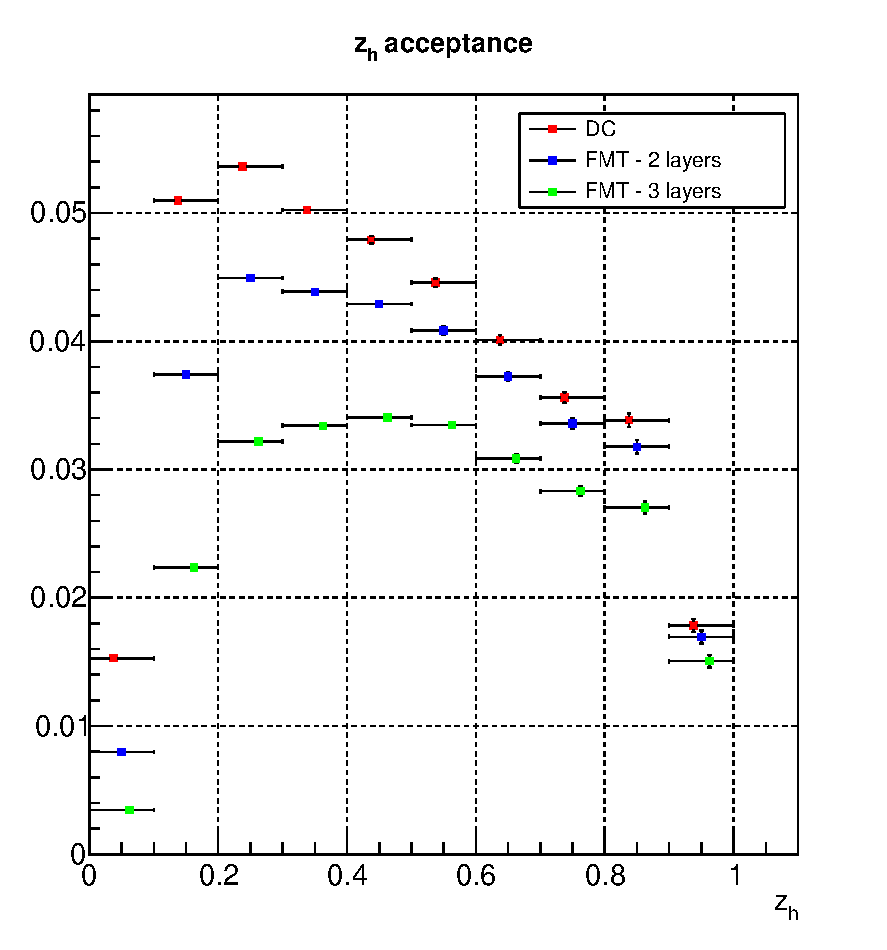
\includegraphics[width=\textwidth]{22zh_acc_211.pdf}
            \caption{$z_h$ acceptance for $e^-\pi^+$.}
            \label{fig::14.22::zh_acc_211}
        \end{subfigure}
        \hfill
        % zh pi-.
        \begin{subfigure}[b]{0.49\textwidth}
            \centering
            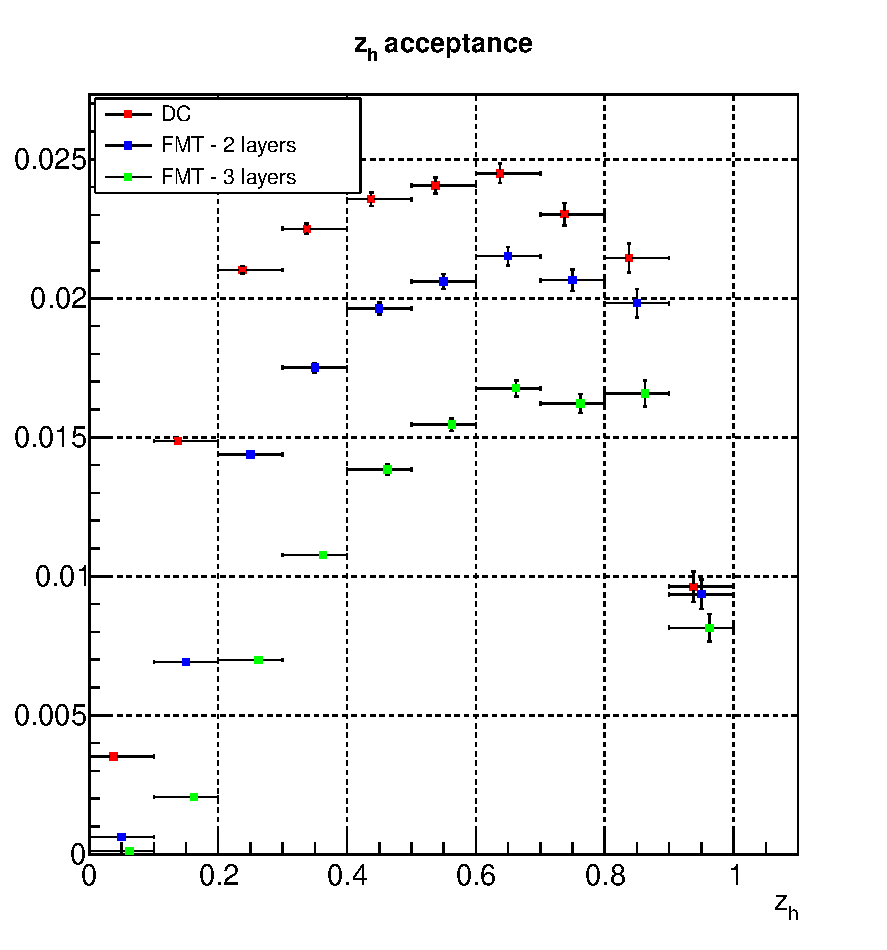
\includegraphics[width=\textwidth]{22zh_acc_-211.pdf}
            \caption{$z_h$ acceptance for $e^-\pi^-$.}
            \label{fig::14.22::zh_acc_-211}
        \end{subfigure}

        \centering
        % pt2 pi+.
        \begin{subfigure}[b]{0.49\textwidth}
            \centering
            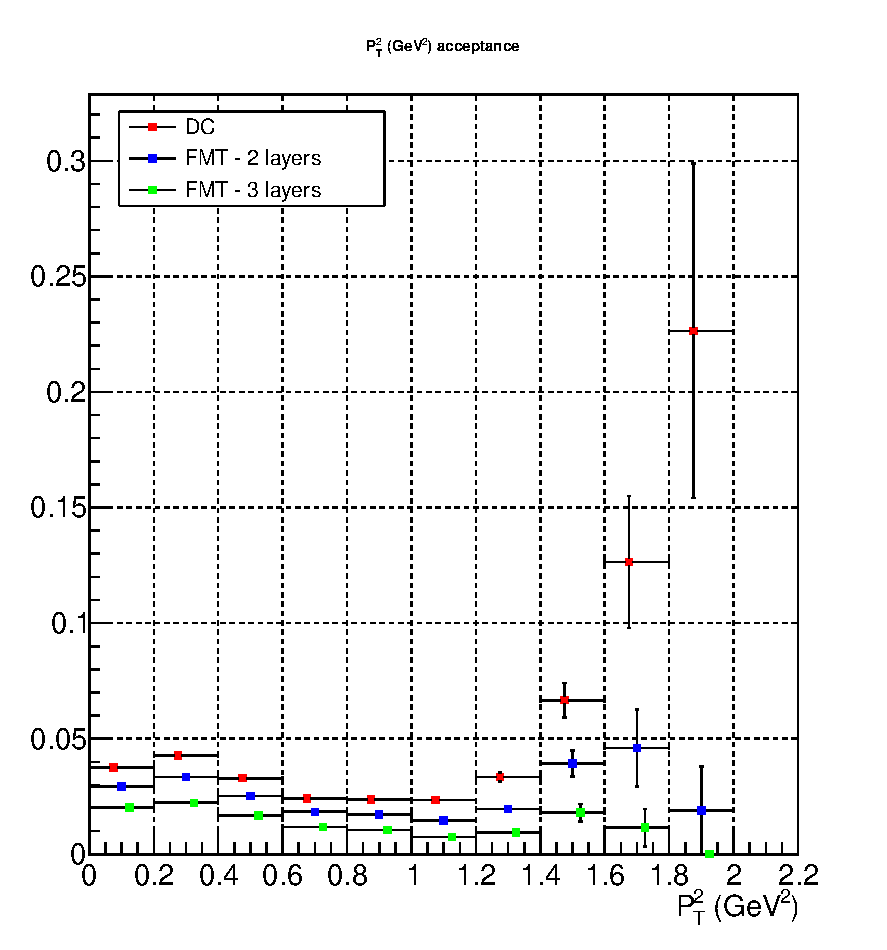
\includegraphics[width=\textwidth]{22pt2_acc_211.pdf}
            \caption{$p_T^2$ acceptance for $e^-\pi^+$.}
            \label{fig::14.22::pt2_acc_211}
        \end{subfigure}
        \hfill
        % pt2 pi-.
        \begin{subfigure}[b]{0.49\textwidth}
            \centering
            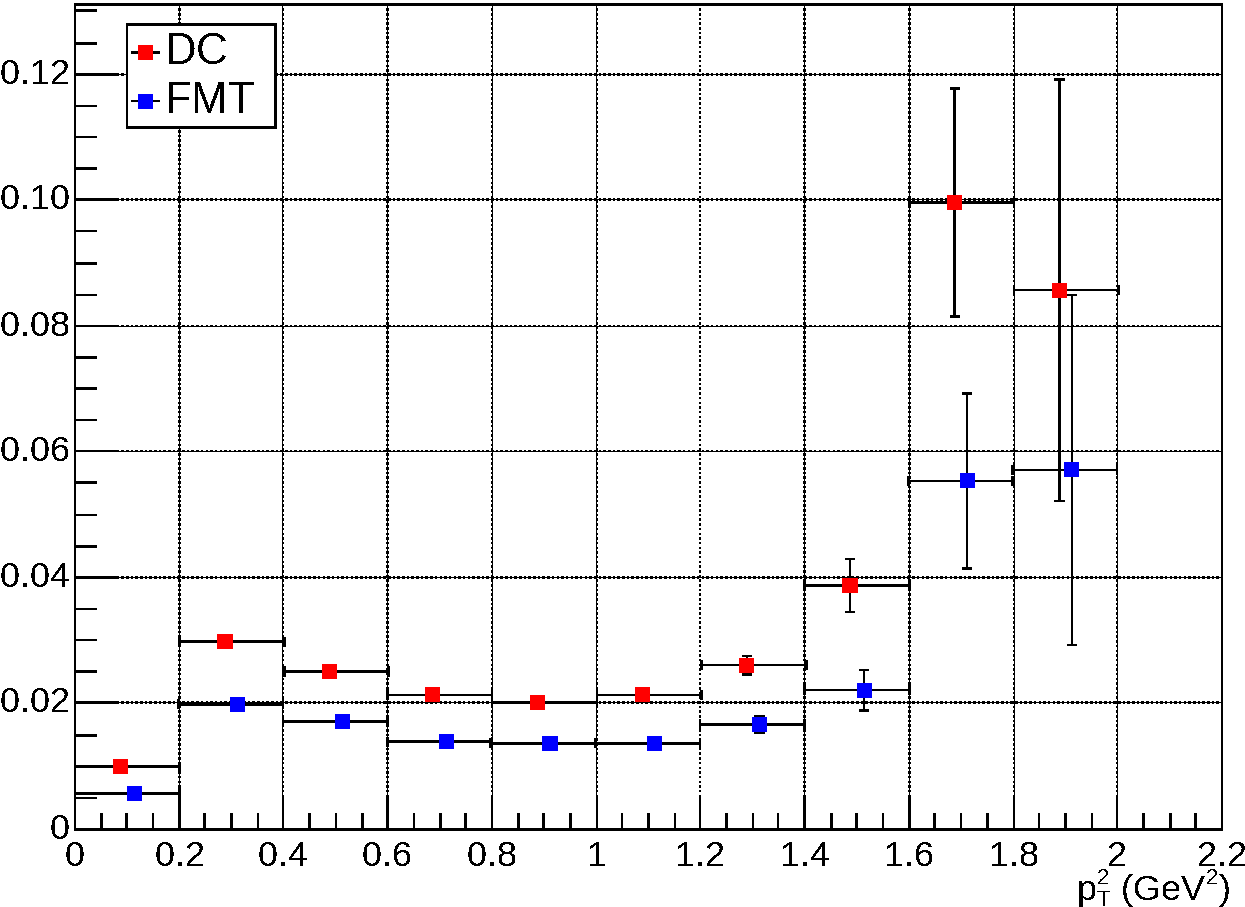
\includegraphics[width=\textwidth]{22pt2_acc_-211.pdf}
            \caption{$p_T^2$ acceptance for $e^-\pi^-$.}
            \label{fig::14.22::pt2_acc_-211}
        \end{subfigure}

        \centering
        % phipq pi+.
        \begin{subfigure}[b]{0.49\textwidth}
            \centering
            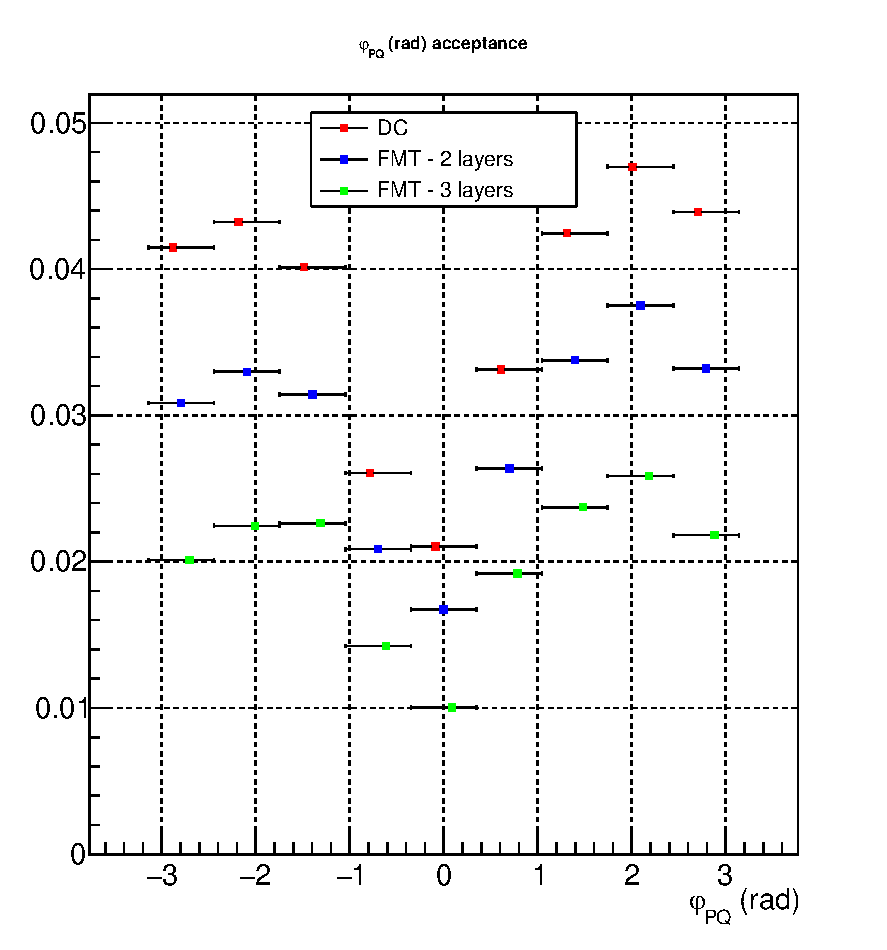
\includegraphics[width=\textwidth]{22phipq_acc_211.pdf}
            \caption{$\phi_{PQ}$ acceptance for $e^-\pi^+$.}
            \label{fig::14.22::phipq_acc_211}
        \end{subfigure}
        \hfill
        % phipq pi-.
        \begin{subfigure}[b]{0.49\textwidth}
            \centering
            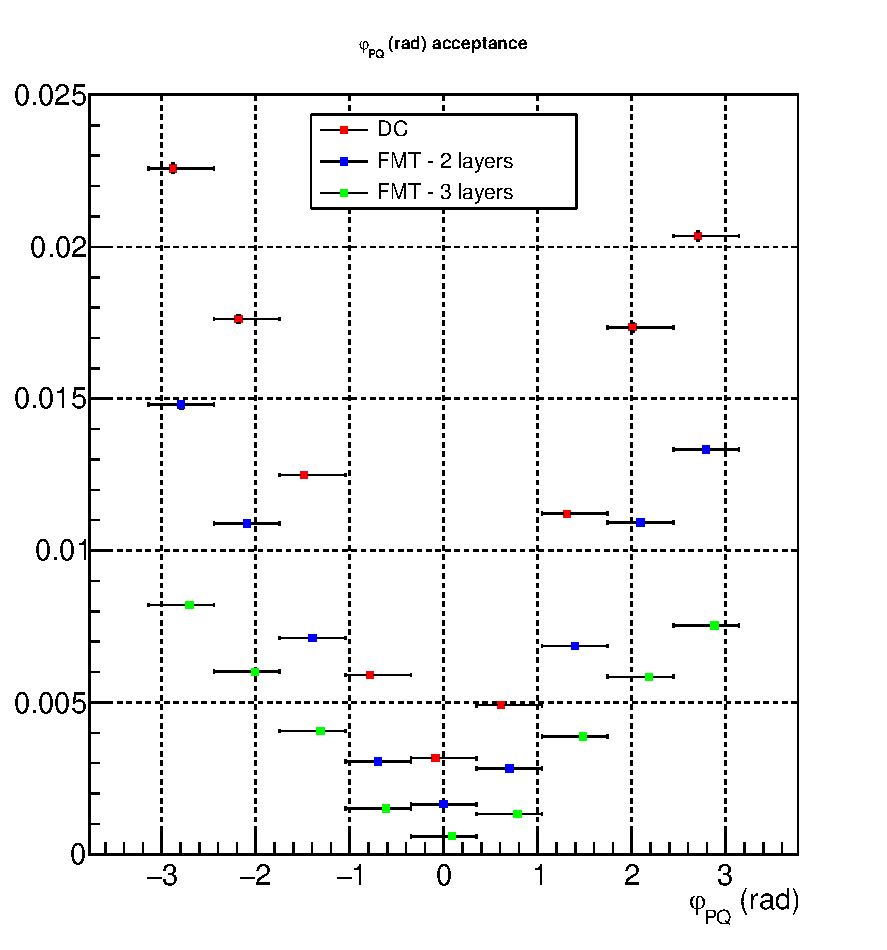
\includegraphics[width=\textwidth]{22phipq_acc_-211.pdf}
            \caption{$\phi_{PQ}$ acceptance for $e^-\pi^-$.}
            \label{fig::14.22::phipq_acc_-211}
        \end{subfigure}
        \caption[Hadronic variables acceptance]
        {$z_h$, $p_T^2$, and $\phi_{PQ}$ acceptances for $e^-\pi^+$ and $e^-\pi^-$.
        All electron and other hadronic variables are integrated in all Figures.
        The bin markers are slightly shifted in $x$ to improve legibility.}
        \floatfoot{Source: Own elaboration, using the \href{https://github.com/bleaktwig/clas12-rge-analysis}{clas12-rge-analysis} software.}
        \label{fig::14.22::hadronic_acc}
    \end{figure}

    \begin{figure}
        \centering
        % phi vs theta.
        \begin{subfigure}[b]{\textwidth}
            \centering
            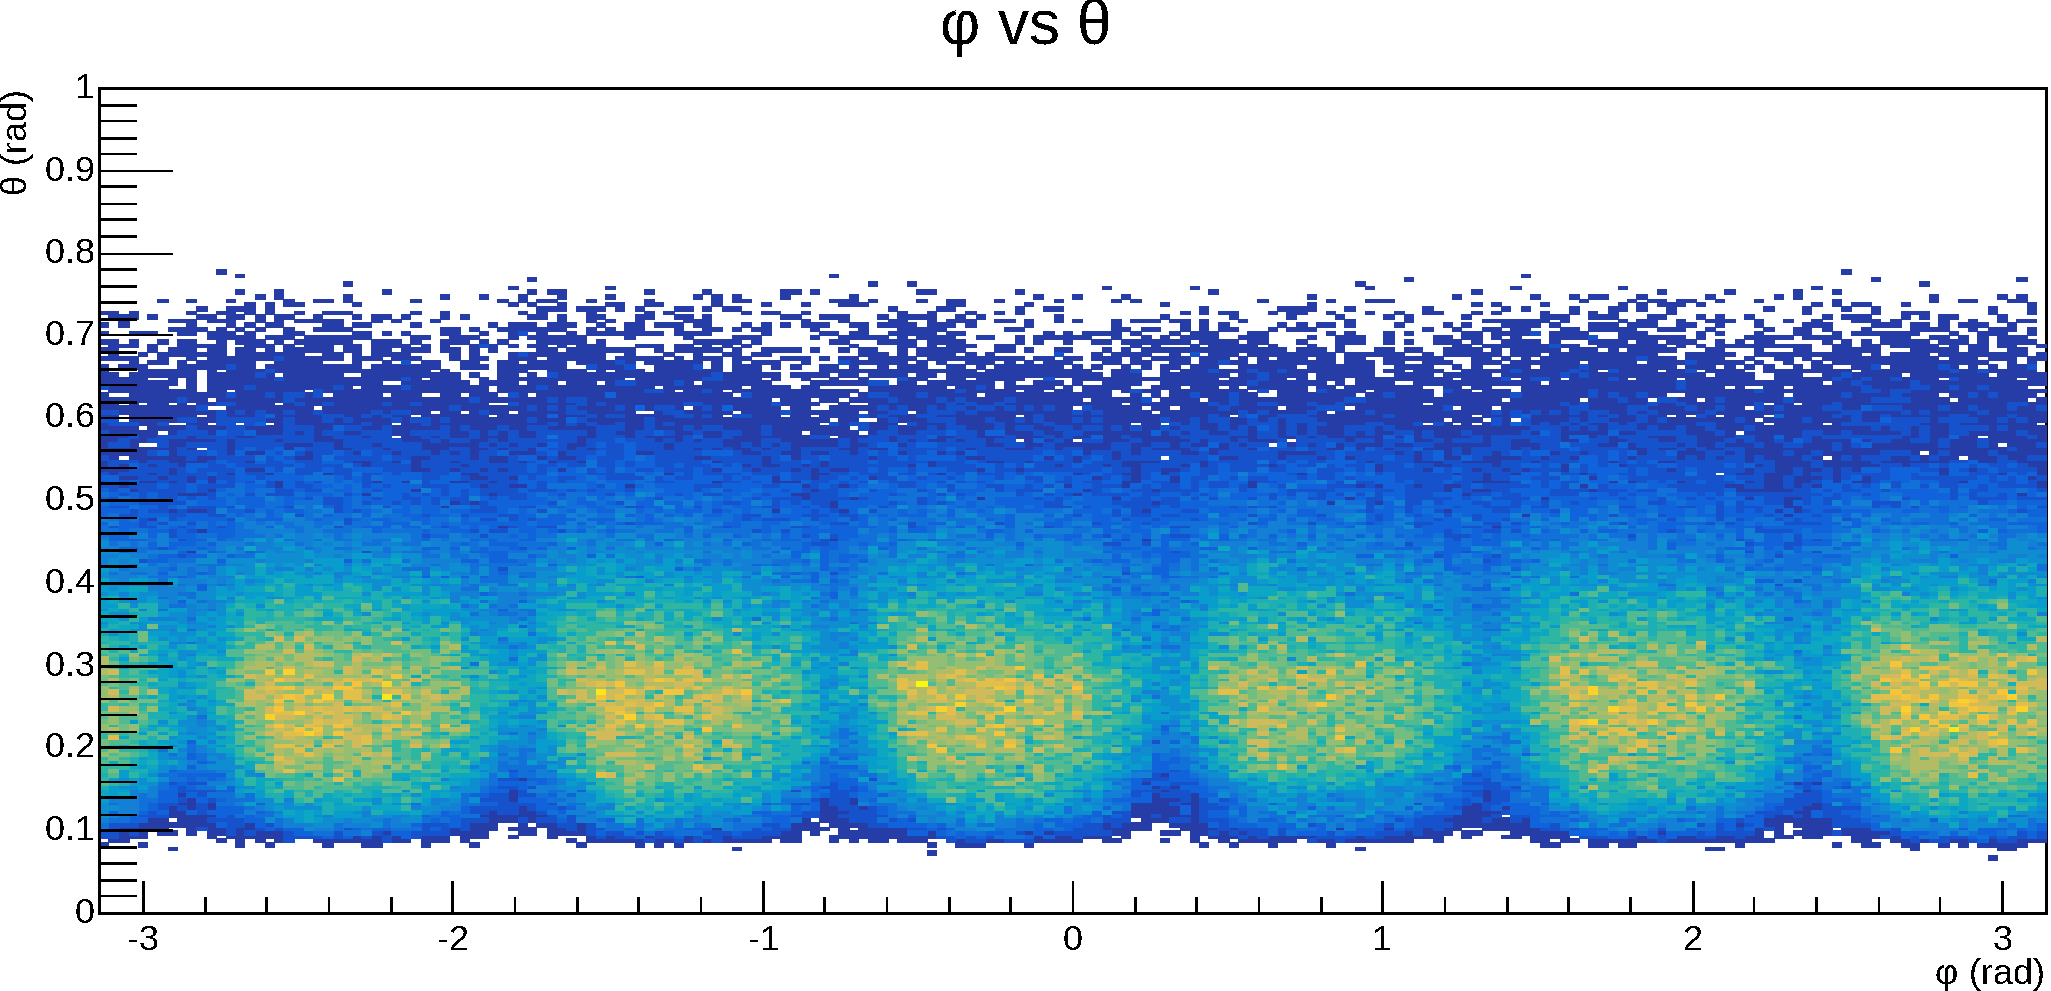
\includegraphics[width=\textwidth]{22phi_theta_pos.pdf}
            \caption[$\phi$ vs $\theta$ for positive particles]
            {$\phi$ vs $\theta$ for positive particles detected by DC.}
            \label{fig::14.22::phi_theta_pos}
        \end{subfigure}
        % theta.
        \begin{subfigure}[b]{\textwidth}
            \centering
            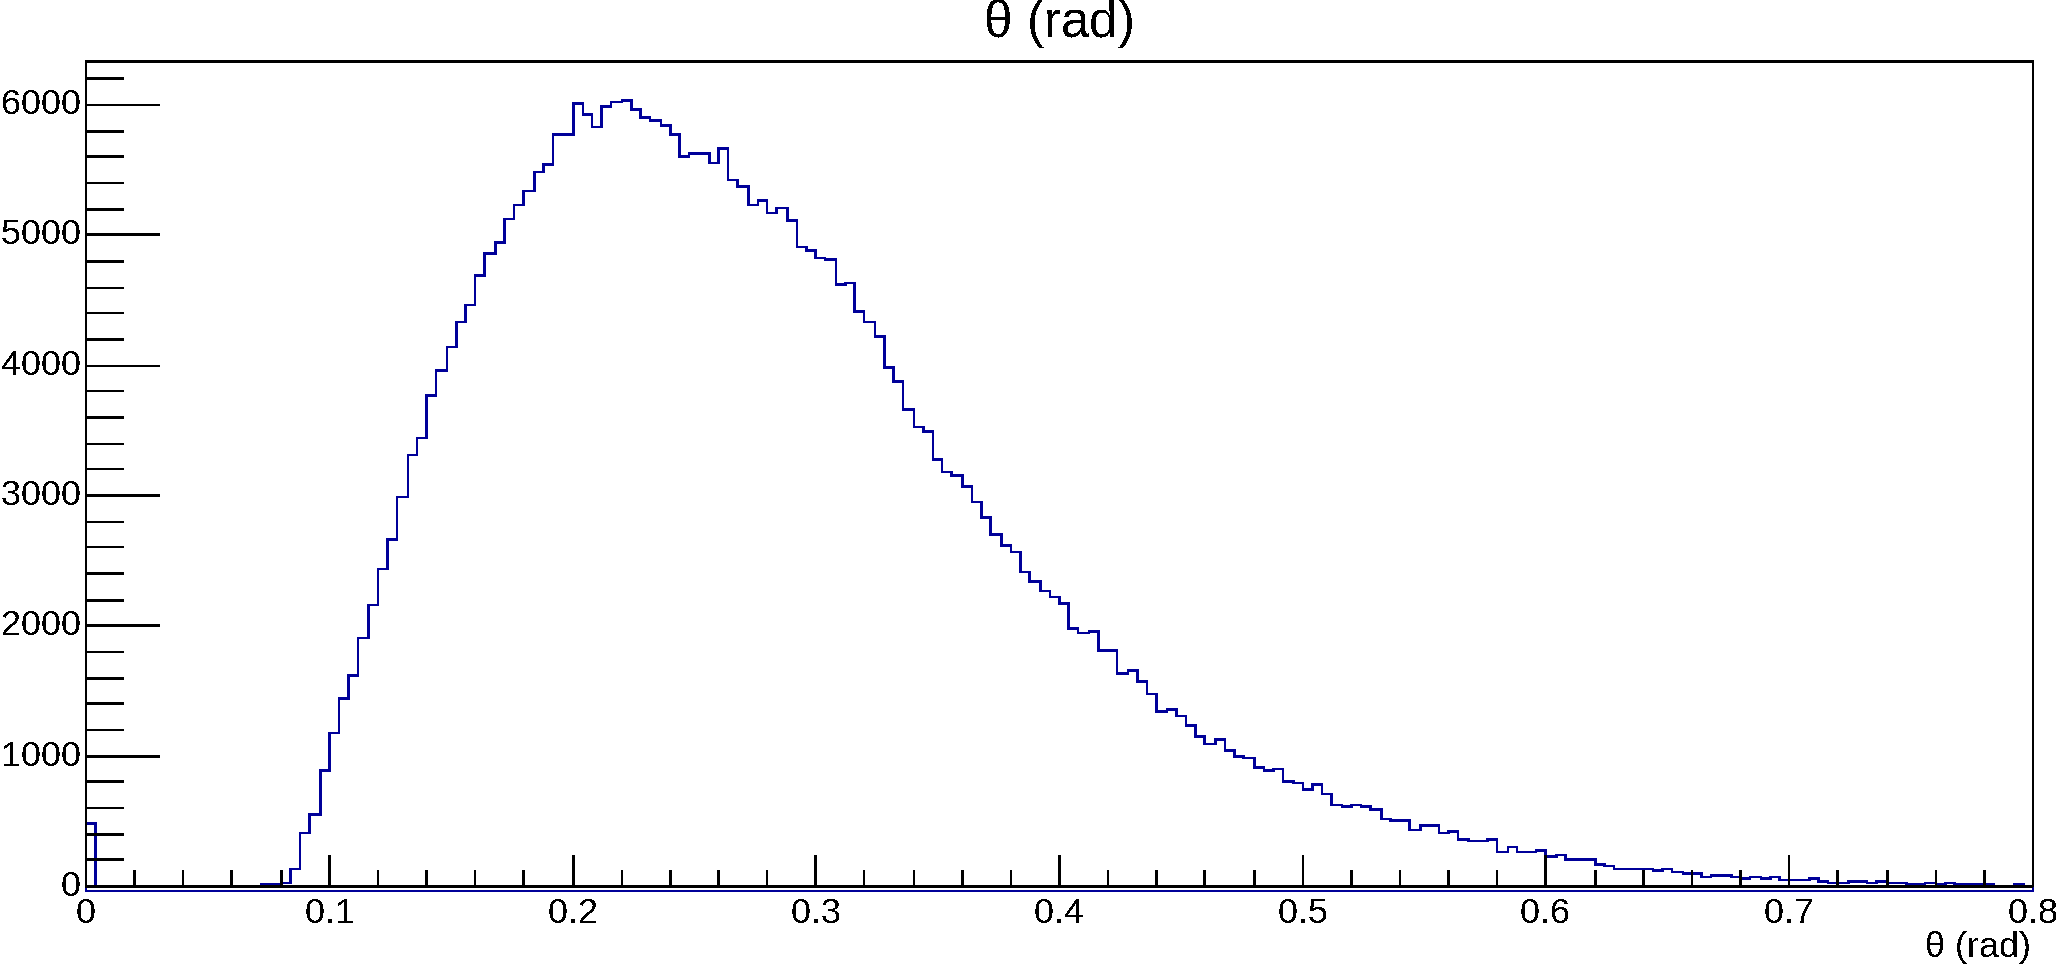
\includegraphics[width=\textwidth]{22theta_pos.pdf}
            \caption[$\theta$ for positive particles]
            {$\theta$ for positive particles detected by DC.}
            \label{fig::14.22::theta_pos}
        \end{subfigure}
        \caption[$\theta$ study for positive particles]
        {$\theta$ study for positive particles.
        Simulated data.}
        \floatfoot{Source: Own elaboration, using the \href{https://github.com/bleaktwig/clas12-rge-analysis}{clas12-rge-analysis} software.}
        \label{fig::14.22::theta_study_pos}
    \end{figure}

    \pagebreak
